\section{Timer opsætning}

Da dronen skal flyve autonomt er det påkrævet at dronen skal styres via main controlleren (arduino boardet). Main controlleren styrer dronen ved at sende 6 forskellige pwm signaler til flight control boardet. De 6 pwm signaler bruges til at kontrollere og regulerer henholdsvis: Throttle, yaw, pitch, roll, alttitudehold og flightmode.

For at undgå at lave busywait når de forskellige pwm signaler skal ændres (skift i periodetid eller duty cycle) benyttes tre 16-bit timere som befinder sig på main controlleren. Arduino 2560 boardet har fire forskellige 16-bit timere, som hver kan styre pwm signal (output signal) på to digitale pins, hvis de  bruges korrekt. 

Fordelen ved at bruge timere til at kontrollere de 6 pwm signaler er primært, at pwm signalerne uafhængig og lynhurtigt kan ændres. For at ændre periodetid eller duty cycle på et pwm signal, skal værdien af et eller flere register blot skiftes. 

PWM signalets periodetiden kan forandres ved at ændre værdien af registeret der bruges til at bestemme hvor højt timeren skal ”tælle”, dette register kaldes typisk TOP eller ICRn. 
PWM signalets duty cycle kan forandres ved at ændre værdien af det register der bestemmer hvornår pwm signalet toggles. Dette register kaldes som regel \textit{Output compare}.

Det blev besluttet at bruge følgende tre timere i Fast PWM mode: \\
Timer1 - til kontrol af de to digitale pins 11 og 12.\\
Timer3 -  til kontrol af de to digitale pins 2 og 5.\\
Timer4 - til kontrol af de to digitale pins 6 og 7. \\

Figur \ref{fig:Timing_diagram} viser hvordan output kan se ud ved brug af en timer i Fast PWM mode.  

%kommentar
\begin{figure}[H]
	\centering
	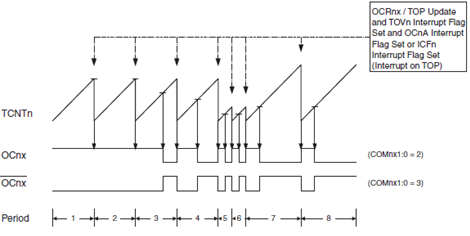
\includegraphics[width=1.\textwidth]{Billeder/Timer/0_timing_diagram.png}
	\caption{Fast PWM Mode, Timing Diagram}
	\label{fig:Timing_diagram}
\end{figure}

\newpage

I det følgende forklares hvordan de tre 16-bit timere er sat op. Bla. forklares valg at mode, udregning af frekvens, samt udregning af hvilke værdier der skal bruges i registerne ICRn og Output compare.

\subsection*{Mode 16-bit timer}

Når main controllerens 16-bits timere benyttes er det muligt at sætte timerne i 16 forskellige modes. Valget af mode styrer dels opløsningen af timeren, men styrer også hvordan timeren skal fungere. Timerne kan bruges i Normal mode, i CTC (Clear Timer on Compare), i Phase Correct PWM Mode eller i Fast PWM.

For at få den størst mulige opløsning benyttes de tre timerne i mode 14 - ”Fast PWM”. I mode 14 bestemmes værdien af TOP, af registeret ICRn som er et 16-bit stort register. Dette betyder at ICRn maksimalt kan sættes til værdien 0xFFFF (65535). 

%kommentar
\begin{figure}[H]
	\centering
	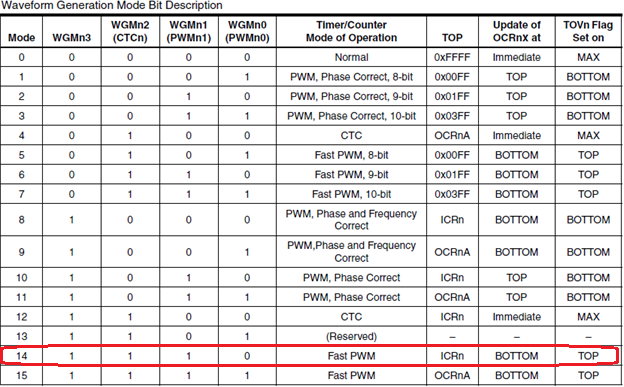
\includegraphics[width=1.\textwidth]{Billeder/Timer/1_mode.png}
	\caption{Fast PWM Mode, Timing Diagram}
	\label{fig:Timing_diagram}
\end{figure}

\newpage

\subsection*{Compare Output Mode}
Når det overordnede mode er valgt for timerne, skal compare output mode vælges. Compare output mode bestemmer hvornår PMW signalet på de forskellige pin sættes helholdvis højt og lavt.

Det besluttes at sætte Compare output mode til:  COMnA1 = 1 og COMnA0 = 0.  Med denne indstilling sættes PWM signalet lavt når timerens counter er lig OCnA eller OCnB og sættes højt igen hver gang timerens counter er lig 0. Indstillingerne sættes på samme vis for COMnB og COMnC.

%kommentar
\begin{figure}[H]
	\centering
	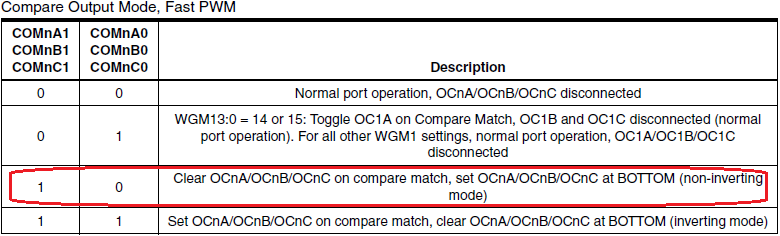
\includegraphics[width=1.\textwidth]{Billeder/Timer/2_compare_output_mode.png}
	\caption{Fast PWM Mode, Timing Diagram}
	\label{fig:Timing_diagram}
\end{figure}

 

\subsection*{TCCR3A}
Da både mode til 16-bit timeren og compare output er valgt kan registeret TCCR3A indstilles. Fra indstilling af mode til 16-bit timeren vides det at WGMn1 = 1, mens WGMn0 = 0. Yderlige vides det at COMnA1 = 1 og COMnA0 = 0 og at COMnB og COMnC skal se ligeledes ud.

Binært skal TCCR3A registeret se således ud: 0b10101010, hvilket i hex svarer til: 0xAA. 

Bemærk: Dette delafsnit tager udgangspunkt i TCCR3A registeret tilhørende timer 3.  TCCR1A og TCCR4A indstilles på samme vis.

%kommentar
\begin{figure}[H]
	\centering
	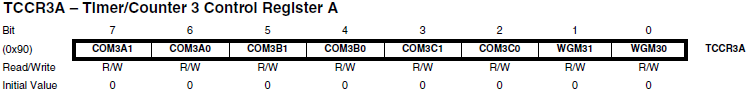
\includegraphics[width=1.\textwidth]{Billeder/Timer/3_TCCT3A.png}
	\caption{Fast PWM Mode, Timing Diagram}
	\label{fig:Timing_diagram}
\end{figure}

\newpage

\subsection*{Clock select}
Hvilken prescale der vælges har betydning for hvor hurtig en clock der bruges til timeren. I udgangspunkt er det en 16MHz clock der bruges, men ved at bruge prescale er det muligt at mindske clocken. Når der gøres brug af en 16-bit timer, har counteren maksimalt 65535 steps. 

Ud fra viden om clockens hastighed og antal steps i counteren kan frekvensen på timernes PWM signal udregnes således: Clock / antal steps = 244,14 Hz.  

Hvilket giver følgende periodetid: 1 / 244,14 Hz = 4,096 ms.

Sættes der prescale på clock’en vil frekvensen falde og periodetiden stige. Men da der ønskes periodetid så tæt på 2ms vælges det ikke at bruge prescale. 

%kommentar
\begin{figure}[H]
	\centering
	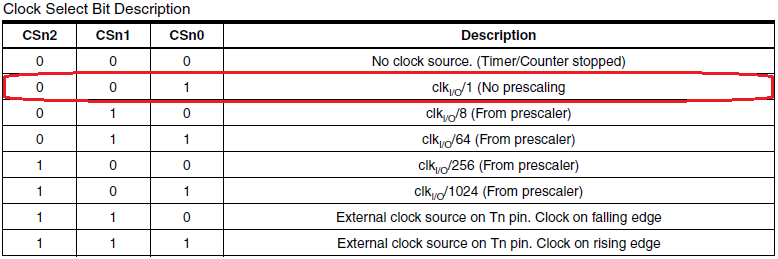
\includegraphics[width=1.\textwidth]{Billeder/Timer/4_CS.png}
	\caption{Fast PWM Mode, Timing Diagram}
	\label{fig:Timing_diagram}
\end{figure}
  

\subsection*{TCCR3B}
Da både mode til 16-bit timeren og clock select er valgt kan registeret TCCR3B indstilles. Fra indstilling af mode til 16-bit timeren vides det at WGMn3 = 1, mens WGMn2 = 1. Yderlige vides det at CSn2 = 0, CSn1 =0 og CSn0 = 1. 

Både ICNC3 (Input Capture Nolse Canceler) og ICES3 (Input Capture Edge Select) sættes lig 0.
Binært skal TCCR3B registeret se således ud: 0b00011001, hvilket i hex svarer til: 0x19. 

Bemærk: Dette delafsnit tager udgangspunkt i TCCR3B registeret tilhørende timer 3.  Registrene TCCR1B og TCCR4B tilhørende timer 1 og 4 indstilles på samme vis.

%kommentar
\begin{figure}[H]
	\centering
	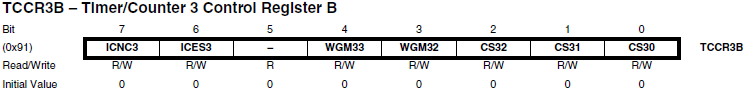
\includegraphics[width=1.\textwidth]{Billeder/Timer/5_TCCT3B.png}
	\caption{Fast PWM Mode, Timing Diagram}
	\label{fig:Timing_diagram}
\end{figure}


\subsection*{TCCR3C}
Force Output Compare A, B og C bruges kun når timeren er sat til et ikke PWM mode.  Derfor sættes Force Output Compare A, B og C = 0.
Binært skal TCCR3B registeret se således ud: 0b00000000, hvilket i hex svarer til: 0x00. 

Bemærk: Dette delafsnit tager udgangspunkt i TCCR3C registeret tilhørende timer 3.  Registrene TCCR1C og TCCR4C tilhørende timer 1 og 4 indstilles på samme vis.

%kommentar
\begin{figure}[H]
	\centering
	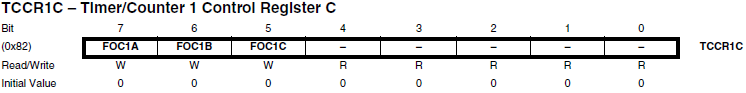
\includegraphics[width=1.\textwidth]{Billeder/Timer/6_TCCT3C.png}
	\caption{Fast PWM Mode, Timing Diagram}
	\label{fig:Timing_diagram}
\end{figure}
 

\subsection*{Indstilling Top og Compare match}
Reelt set er opsætningen af duty cycle og periodetid fuldstændig ligegyldigt. Det eneste der betyder noget, er at de PWM signaler der sendes til flight control boardet har pulsbredde mellem 1-2 ms.
 
Det vides at periodetiden på pwm signalerne vil være 4,096 ms når der arbejdes med clock på 16MHz, der ikke benyttes prescale og Top = 65535.

Ved opstilling af to simple ligninger, kan det beregnes hvilken værdi der skal skrives ind i compare match registeret for at skabe et pwm signal med pulsbredde på 1 ms.  

4,096 ms * x = 1 ms	Udtrykket omformes til: 	x = 1 ms / 4,096 ms = 0,244.

Værdi af Compare match for at opnå pulsbredde på 1ms:  Top * x = 65535 * 0,244 ~ 16000.

På samme vis kan det udregnes hvilken værdi der skal skrives i compare match for at få pulsbredde på 2 ms.

4,096 ms * x = 2 ms	Udtrykket omformes til: 	x = 2 ms / 4,096 ms = 0,488

Værdi af Compare match for at opnå pulsbredde på 1ms:  Top * x = 65535 * 0,488 ~ 32000.

Det er nu beregnet: Pulsbredde på 1ms fås ved compare match = 16000, mens pulsbredde på 2ms fås ved compare match = 32000. For at styre flight control board skal værdien i compare match altså veksle op og ned i størrelse mellem 16000 og 32000. 






